\chapter{Aritmetica Modulare}
L'\textit{aritmentica modulare} è un settore della matematica che si occupa dello studio di particolari \textbf{insiemi numerici} e delle \textbf{operazioni} definite su di essi. Gli insiemi oggetto di studio sono sottoinsiemi finiti dei numeri interi, ciascuno definito tramite un intero positivo \textit{n}, detto \textbf{modulo} $\Rightarrow$ $\mathbb{Z}_n$. 
\newline
$\mathbb{Z}$ $\Rightarrow$ insieme matematico per i numeri interi positivi.
\newline
$\mathbb{Z}_n = \{0, 1, ..., n-1\}$ $\Rightarrow$ può essere visto come l'insieme dei \textbf{\textit{possibili resti}} quando si divide un numero intero per \textit{n}.
\\ \newline
\textbf{Note Terminologiche}
\newline
$y \bmod n = x \bmod n$ $\Rightarrow$ \textit{x} è congruo $y \bmod n$, anche rappresentato come: $x \equiv y \bmod n$.
\newline
$\Rightarrow$ implica che il resto di $\frac{x}{n}$ e $\frac{y}{n}$ siano uguali, avremo quindi che $x - y = kn$.
\\ \newline
\textbf{Operazioni Modulari}
\newline
Negli insiemi $\mathbb{Z}_n$ sono definite quattro operazioni aritmetiche: 
\begin{center}
    $Op_n = \{+, -, \times, \div\}$ $\Rightarrow$ Nel caso della $\div$ sarà necessaria una condizione affinché sia garantita all'interno di un gruppo $\mathbb{Z}_n$. 
\end{center}
Indicheremo con $+_n$ la somma modulare. Ogni operazione coincide con la medesima operazione sugli interi seguita dal calcolo del resto modulo \textit{n}. Se indichiamo con \textbf{\textit{Q}} e \textbf{\textit{R}} rispettivamente il quoziente e il resto della divisione $\frac{a}{b}$ deve valere:
\begin{center}
    $a = b \cdot Q + R \rightarrow R \in \{0, 1, ..., b - 1\}\;\;\;(0 \le R < b)$
\end{center}
Questa condizione deve essere sempre rispettato, anche quando il resto è negativo. Bisogna guardare il rappresentante del gruppo $\mathbb{Z}_n$.
\begin{center}
    $-1 \bmod N = N -1$ $\Rightarrow$ $\mathbb{Z}_n$ è chiuso rispetto alle operazioni definite su di esso.
\end{center}
\   \\
\textbf{Elemento Neutro e Inverso in $\mathbb{Z}_n$} 
\newline
Nel gruppo \textbf{additivo} ${\mathbb{Z}_n}^+$ avremo:
\begin{itemize}
    \item 0 è l'elemento \textbf{neutro}.
    \item l'opposto di $x \in {\mathbb{Z}_n}^+$ è l'\textbf{inverso additivo} ed è calcolabile come:
    \begin{center} 
        $z \in {\mathbb{Z}_n}^+\;|\; x +_n z = 0 \;\;\;\Rightarrow \;\;\; z = n - x$
    \end{center}
\end{itemize}
Per parlare invece dei due elementi: \textbf{neutro} e \textbf{inverso} nel gruppo \textbf{moltiplicativo} ${\mathbb{Z}_n}^*$ è necessario chiarire la condizione per poter dividere all'interno del nostro gruppo $\mathbb{Z}_n$. Negli insieme $\mathbb{Z}_n$ la divisione non può essere definita a partire dalle corrispondenti operazioni sugli interi, perché
\begin{center}
    in $\mathbb{R}$ se $x = \frac{a}{b}$ $\Rightarrow$  $a * {1 \over b}$
    \   \\ 
    Dove $\frac{1}{b}$ è l'\textbf{inverso moltiplicativo} di \textit{a} in $\mathbb{R}$, ma in aritmetica modulare e più precisamente in $\mathbb{Z}_n$ non è sempre definito l'inverso moltiplicativo di \textit{b}, con $b \in \mathbb{Z}_n$.
\end{center}
Definiamo invece l'\textbf{inverso moltiplicativo} di un elemento $x \in \mathbb{Z}_n$ quel numero \textit{z}, se esiste:
\begin{center}
    $x \times_n z = (x * y) \bmod n = 1$ \\
    $\exists z, \;z \in \mathbb{Z}_n \iff gcd(z, n) = 1$
\end{center}
Andando a definire che il valore \textit{z} esiste all'interno del gruppo $\mathbb{Z}_n$ se e solo se l'\textbf{\textit{MCD}}(\textit{z}, \textit{n}) è pari a 1, ovvero se e solo se \textit{z} e \textit{n} sono \textbf{realtivamente primi} tra di loro (\textbf{coprimi}).
\newline
$\Rightarrow$ se \textit{n} è un numero \textbf{primo}, allora per ogni elemento appartenente a $\mathbb{Z}_n \textbackslash \{0\}$ avrà un \textbf{inverso moltiplicativo}
\begin{center}
    se $n = p$ $\Rightarrow$ $\forall x \in \mathbb{Z}_p$, $\exists z \in \mathbb{Z}_p\;|\; (x * z) \bmod p = 1$
\end{center}

\textbf{\textit{Identità di BEZOUT}}
\newline
Dati due numeri interi \textit{x} e \textit{n}, non entrambi nulli, esistono due numeri interi \textit{a} e \textit{b} tali che: $gcd(x, n) = a * x + b * n$. Inoltre \textbf{MCD}(\textit{x}, \textit{n}) è il più piccolo intero positivo esprimibile come combinazione lineare di \textit{x} e \textit{n}.
\begin{figure}[h]
    \begin{minipage}[t]{0.45\textwidth}
        \textbf{1.} $gcd(x, n) = 1$ \\
        \textbf{2.} $1 = a * x + b * n$ \\
        \textbf{3.} $a * x = 1 - n * n$ \\
        \textbf{4.} $(a * x) \bmod n = 1 - (b * n) \bmod n$ \\
        \textbf{5.} $(a * x) \bmod n = 1$
    \end{minipage}
    \hfill
    \begin{minipage}[t]{0.45\textwidth}
        \textbf{1.} Dimostriamo che solo se \textit{x} e \textit{n} sono primi allora esiste l'inverso di \textit{x} \\
        \textbf{2.} Applichiamo l'\textit{identità di bezout} \\
        \textbf{4.} Applichiamo il modulo a destra e a sinistra \\
        \textbf{5.} $(b * n) \bmod n$ è 0 perché $b * n$ è multiplo di \textit{n} e quindi il resto della divisione per \textit{n} è 0.
    \end{minipage}
\end{figure}
\   \\
In questo caso vediamo che \textit{a} ha la stessa proprietà di \textit{z} ovvero che è l'inverso di $x \in \mathbb{Z}_n$. Avremo quindi che $a \equiv x^{-1} \bmod n$.
\\ \newline
\textbf{Calcoli in} $\mathbb{Z}_n$
\newline
Supponiamo di dover calcolare un espressione $\epsilon_{\mathbb{Z}_n}$ in $\mathbb{Z}_n$ cioè un espressione in cui tutte le operazioni sono modulari e sia $\epsilon_{\mathbb{Z}}$ la corrispondente espressione in $\mathbb{Z}$ vale:
\begin{center}
    $\epsilon_{\mathbb{Z}_n} = \epsilon_{\mathbb{Z}} \bmod n$
\end{center}
$\Rightarrow$ eseguire il calcolo del resto solo sull'ultimo valore calcolato (vale anche il contrario: è possibile portar eil modulo osu qualsiasi valore intermedio).
\newline
Se \textit{m} divide \textit{n} allora per qualsiasi valore $x \in \mathbb{Z}_n$ allora $(x \bmod n) \bmod m = x \bmod m$.
\\ \newline
Gli \textbf{Algoritmi di Euclide} ed \textbf{Euclide Esteso}
\newline
L'\textit{algoritmo di Euclide Esteso} costituise un metodo \textbf{efficente} per calcolare l'\textit{inverso moltiplicativo} di un elemento $x \in \mathbb{Z}_n$ se esiste.
\newline
Partiamo, per semplicità enunciando l'\textit{algoritmo di Euclide} che permette di calcolare il massimo comune divisore (\textbf{\textit{MCD}}) di due numeri interi. L'algoritmo è basato sull'ugualianza: $gcd(x, y) = gcd(y, x \bmod y),\;\;\;y\neq0$ che unito alla ``condizione base'' $gcd(x, 0) = x$ nel caso in cui \textit{y} sia nulla permette di \textbf{definire per ricorrenza} il teorema:
\begin{center}
    \begin{math}
        gcd(x, y) = 
        \begin{cases}
            x \qquad \qquad \qquad \qquad y = 0 \\
            gcd(y, x \bmod y) \qquad y \in \mathbb{Z} \textbackslash \{0\}
        \end{cases}
    \end{math}
\end{center}
\   \\ \newline
\textcolor{red}{\textbf{DIMOSTRAZIONE}}: dobbiamo dimostrare che le seguenti equazioni siano verificate nello stesso momento: $gcd(x, y) \leq gcd(y, x \bmod y)$ e $gcd(y, x \bmod y) \leq gcd(x, y)$. Consideriamo:
\begin{enumerate}
    \item se un numero \textit{m} divide \textit{x} e \textit{y} allora divide una qualsiasi \textbf{combinazione linerare} a coefficenti interi \textit{x} e \textit{y}.
    \begin{center}
        $ m|a \land m|b \Rightarrow m|(a*x + b*y)\;\;a,b\in\mathbb{Z}$
    \end{center}
    \item $x \bmod y$ è una combinazione linerare di \textit{x} e \textit{y}.
    \begin{center}
        $x \bmod y = x - \floor{\frac{x}{y}} * y = R$
    \end{center}
\end{enumerate}
Poiché $gcd(x, y)$ divide sia \textit{x} che \textit{y}, ma anche qualsiasi combinazione lineare a coefficenti interi \textit{x} e \textit{y}, quindi $a = 1, b = \floor{\frac{x}{y}}$ per cui vale che $a,b \in \mathbb{Z}$. Avremo che il $gcd(x, y)$ divide $x - \floor{\frac{x}{y}} * y$ che non è altro che $x \bmod y$, ma divide anche \textit{y}. Ne consegue:
\begin{center}
    $gcd(x, y)\;|\;x \bmod y$ \\
    $gcd(y, x \bmod y)$ è il valore massimo fra i divisori comuni tra \textit{y} e $x \bmod y$ \\
    $gcd(y, x \bmod y) \geq gcd(x, y)$ 
\end{center}
\   \\
Poiché $gcd(y, x \bmod y)$ divide sia \textit{y} che $x \bmod y$ allora divide anche qualsiasi combinazione lineare a coefficenti interi di \textit{y} e $x \bmod y$. Per questo secondo caso dovremo tenere conto della combinazione lineare: $x = y * Q + R$ dove $Q = \floor{\frac{x}{y}}$, ne consegue:
\begin{center}
        $gcd(y, x \bmod y)\;|\; x$  \\
        $gcd(y, x \bmod y)\;|\; y * Q + R$  \\
        $gcd(y, x \bmod y)\;|\; y * \floor{\frac{x}{y}} + (x \bmod y)$
\end{center}
\begin{center}
    \begin{math}
        \begin{aligned}
            x& = a * y + b * x \bmod y = a * y + b * (x - \floor{\frac{x}{y}} * y) \\
            & = \floor{\frac{x}{y}} * y + 1 * (x - \floor{\frac{x}{y}} * y)
        \end{aligned}    
    \end{math}
\end{center}
\begin{center}
    $gcd(x, y) \geq gcd(y, x \bmod y) $
\end{center}
\   \\
\textbf{Algoritmo di Euclide Esteso}
\newline
Possiamo modificare la ricorsione del metodo di Euclide in modo da calcolare oltre che $gcd(x, y) = m$ anche i due valori interi tali \textit{a} e \textit{b} che soddisfano l'\textbf{identità di \textit{Bezout}}:
\begin{center}
    $m = a * x + b * y$ \\
\end{center}
1. caso base: $y = 0\;\;\; m = a * x + 0 = 1 * x = m$, ottenendo, quindi, $a = 1$ e $b = 0$, possiamo quindi definire la formula generale della ricorrenza tramite:
\begin{center}
    \begin{math}
        EEuclide(x, y) =
        \begin{cases}
            x, 1, 0 \qquad \qquad \qquad y = 0 \\
            m, b, a - b * \floor{\frac{x}{y}} \qquad m, a, b = EEuclide(y, x \bmod y)
        \end{cases}
    \end{math}
\end{center}
\   \\ \newline
\textcolor{red}{\textbf{DIMOSTRAZIONE}}: attraverso \textit{ipotesi induttiva}.
\\ \newline
\begin{math}
    \begin{aligned}
        m& = gcd(x, y) = gcd(y, x \bmod y) = a * x + b * y \\
        & = a * y + b * x \bmod y = a * y + b * (x - \floor{\frac{x}{y}}) \\
        & = a * y + b * x - b * \floor{\frac{x}{y}} * y \\
        m& = b * x + (a - b * \floor{\frac{x}{y}}) * y
    \end{aligned}
\end{math}
\   \\ \newline
\textbf{Calcolo dell'inverso}
\newline
Possiamo utilizzare l'algoritmo di \textit{euclide esteso} per il calcolo dell'inverso moltiplicativo di $x \bmod n$:
\begin{center}
    $m, a, b = EEuclide(x, n)$ \\
    \begin{math}
        x ^ {-1} \bmod n =
        \begin{cases}
            0 \qquad \qquad \qquad m > 1 \\
            a \bmod n \qquad\;\;\; m = 1
        \end{cases}
    \end{math}
\end{center}

\textbf{Teorema Cinese dei Resti}
\newline
È lo strumento teorico per cui è possibile ridurre il tempo di computazione nelle operazioni di crifratura (\textit{RSA}) e decifratura. Definiamo \textit{n} un numero intero esprimibile come prodotto di $r > 1$ numeri interi tra di loro \textbf{coprimi}.
\begin{center}
    $n = n_1 * n_2 * ... * n_r$
\end{center}
Allora il resto della divisione di un qualsiasi numero intero \textit{a} per \textit{n}, ovvero $a \bmod n$ è \textbf{completamente determinato} dai resti delle divisioni per $n_1, n_2, ..., n_r$. In altri termini esiste una \textbf{corrispondenza biunivoca} fra $Z_n$ e il \textbf{prodotto cartesiano} $Z_{n_1} \times Z_{n_2} \times ... \times Z_{n_r}$.
\newline
\begin{math}
    a \in \mathbb{Z}_n \qquad a \rightarrow (a_1, a_2, ..., a_r) \rightarrow (a \bmod n_1, a \bmod n_2, ..., a \bmod n_r) \\
    c = c_1 * a_1 + c_2 * a_2 + ... + c_r * a_r \qquad c_i \in {0, 1} \rightarrow C \bmod n_i = a_i \\
    m_i = \prod_{j \ne i} n_i \qquad \Rightarrow \text{prodotto di tutti i moduli ad eccezione proprio dell'i-esimo } n_i \\
    gcd(m_i, n_i) = 1 \;\;\; \Rightarrow \text{per il passaggio di costruzione di } m_i \\ \\
    c_i = m_i * ({m_i}^{-1} \bmod n_i) \Rightarrow c_i \bmod n_j = 0, c_i \bmod n_i = 1 \\ \\
    C = \sum_{i = 1}^r c_i * a_i \qquad \Rightarrow c \bmod n_i = a_i, \;\;\; i = 1, ..., r \\
    C \bmod n = a \bmod n \Rightarrow C = a \text{ hanno la stessa rappresenzatione in } \mathbb{Z}_n
\end{math}
\   \\ \newline
\textbf{Gruppi e Gruppi Ciclici} $\mathbb{Z}_n \text{ e } {\mathbb{Z}_n}^{*}$
\newline
L'operazione $\{+_n\}$ in $\mathbb{Z}_n$ gode delle seguenti proprietà:
\begin{enumerate}
    \item \textbf{Chiusura}: la somma (modulare) di due elementi in $\mathbb{Z}_n$ è ancora un elemento di $\mathbb{Z}_n$: $z = x +_n y \; \exists z \in \mathbb{Z}_n, \forall x,y \in \mathbb{Z}_n$
    \item \textbf{Associativa}: $(a +_n b) +_n c = a +_n (b +_n c)$
    \item \textbf{Esistenza dell'Elemento Neutro}: 0
    \item \textbf{Esistenza dell'Elemento Inverso} $x \in \mathbb{Z}_n \rightarrow x^{-1} = n - x$
\end{enumerate}
In questo modo possiamo dire che $\mathbb{Z}_n$ è un \textbf{gruppo} rispetto alla somma modulare.
Consideriamo ora l'operazione $\{{\times}_n\}$ e consideriamo sempre l'insieme $\mathbb{Z}_n$ allora $\exists \; x^{-1} \in \mathbb{Z}_n \iff gcd(x, n) = 1$. \\
Se \textit{x} e \textit{n} non sono coprimi non esiste l'inverso di \textit{x} in $\mathbb{Z}_n$ e quindi $\mathbb{Z}_n$ non è un gruppo rispetto alla moltiplicazione (modulare). ${\mathbb{Z}_n}^{*}$ è il gruppo moltiplicativo in \textit{n} composto da tutti quegli elementi $x \in \mathbb{Z}_n\;|\; gcd(x, n) = 1$.
\\ \newline
\textcolor{green}{\textbf{Es.}} \\
$\mathbb{Z}_{12}^* \ne \mathbb{Z}_{12} \Rightarrow \{1, 5, 7, 11\} \neq \{1, 2, 3, 4, 5, 6, 7, 8, 9, 10, 11\}$
\\ \newline
\textbf{Se \textit{n} è primo $\mathbb{Z}_n$ è un campo}
\newline
$\mathbb{Z}_p = \{0, 1, ..., p - 1\}\;\Rightarrow$ conserva tutte le proprietà per essere un gruppo additivo (chiusura, associativa, esistenza dell'elemento neutro e inverso rispetto alla somma). 
\newline
Siccome \textit{p} è primo. Presenta tutti gli inversi $\forall x \in \mathbb{Z}_n$, perché $\forall x \in \mathbb{Z}_p \exists x^{-1} \in \mathbb{Z}_p \rightarrow gcd(x, p) = 1 \;\; \forall x \in \mathbb{Z}_p$ (chiusura, proprietà associativa, esistenza dell'elemento neuto, 1, e inverso rispetto alla moltiplicazione).
\newline
$\mathbb{Z}_p$ presenta anche la proprietà \textbf{distributiva} poiché $\mathbb{Z}_p$ è sia un gruppo \textit{additivo} che \textit{moltiplicativo}. In questo caso $\mathbb{Z}_p$ è un \textbf{Campo Finito}, in matematica definiamo \textit{campo} una struttura algebrica composta da un insieme non vuoto e da duue operazioni binarie intere: somma e prodotto. Un \textbf{Campo Finito} viene anche chiamato: \textbf{Campo di \textit{Galois}}.
\\ \newline
\textbf{Ordine di un elemento in un gruppo}
\newline
Viene definito \textit{ordine} di \textit{x} appartenente ad un gruppo il numero che rappresenta il minimo numero di volte che dobbiamo fare $\{Op.\} x$ per ottenere l'elemento neutro, partedo dall'elemento neutro stesso.
\begin{itemize}
    \item \textbf{Gruppi Additivi}: $ord(x), x \in \mathbb{Z}_n \Rightarrow x * ord(x) \bmod n = 0$
    \item \textbf{Gruppi Moltiplicativi}: $ord(x), x \in {\mathbb{Z}_n}^* \Rightarrow x^{ord(x)} \bmod n = 1$ 
\end{itemize}
\   \\ 
\textbf{Gruppi Ciclici e Generatori}
\newline
Il numero di elementi di un gruppo \textit{G} è detto \textbf{ordine di \textit{G}}, un gruppo si dice \textbf{ciclico} se esiste almeno un elemento $g \in G$ che abbia ordine pari all'ordine del gruppo.
\begin{center}
    $ord(g) = ord(G)$
\end{center}
\textit{g} se è verificata l'ugualianza precedente è detto \textbf{generatore} o anche \textbf{radice primitiva} di \textit{G}.
\newline
I gruppi additivi $\mathbb{Z}_n$ e moltiplicativi $\mathbb{Z}_n^*$ con \textit{n} primo sono \textbf{gruppi ciclici}, infatti se \textit{g} è un generatore vale:
\begin{center}
    $\mathbb{Z}_n^* = \{g^i \bmod p | i = 1, ..., p - 1\}$    
\end{center}
Consideriamo un elemento di \textit{h} di ordine \textit{s} con $s < | \mathbb{Z}_n^* | $ (ovvero non un generatore, nel caso di \textit{n} primo avremo che la \textbf{cardinalità} è $p - 1$) possiamo comunque considerare l'insieme \textit{H} generato da \textit{h}:
\begin{center}
    $H = \{h^i \bmod p | i = 1, ..., s\}$
\end{center}
\textit{H} è un sottogruppo ciclico di $\mathbb{Z}_p^*$ (ogni sottogruppo deve sempre includere l'elemento 1, infatti è l'elemento neutro di un gruppo moltiplicativo).
\begin{center}
    $x = h^i \bmod p \;\;\; i \leq s \Rightarrow$ $s - i$ è l'inverso di \textit{i} \\
    $x^{-1} \bmod p = h^{s-i} \bmod p\;\Rightarrow$ moltiplico per gli inversi \\
    $x*x^{-1} \bmod p = h^i*h^{s-i} \bmod p\;\Rightarrow$ sostituisco \\
    $h^i * xx^{-1} \bmod p = h^i * h^{s-i} \bmod p$ \\
    $x^{-1} \bmod p = h^{s-i} \bmod p$ \\
    $x \text{ ha inverso moltiplicativo } h^{s-i} \bmod p$
\end{center}
\   \\
\textbf{Teorema di Lagrange}: Qualsiasi sottogruppo di un gruppo di ordine \textit{k} ha necessariamente ordine che è un divisore di \textit{k}.
\\ \newline
\textbf{Teorema Fondamentale dei Gruppi Ciclici}: Per ogni divisore \textit{k} dell'ordine del gruppo esiste uno ed uno solo sottogruppo di ordine \textit{k}. Ovvero se 2 o più generatori \textit{h} di sottogruppi di $\mathbb{Z}_p^*$ con uguale ordine (o cardinalità) $\Rightarrow$ allora quei due generatori genereranno lo stesso sottogruppo.
\begin{center}
    $H = \{h^i \bmod p | i = \{1, ..., s\}\}$ \\
    $H' = \{h'^i \bmod p | i = \{1, ..., s\}\}$ \\
    $ord(H) = ord(H') \Rightarrow H = H'$ \\    
\end{center}
\   \\
\textbf{\textit{Strong Prime}} o \textbf{\textit{Safe Prime}}: i \textit{safe prime} vengono definiti come $p = 2*q + 1$ dove anche \textit{q} è un numero primo. Per il teorema di \textit{Lagrange} l'ordine dei sottogruppi non banali può essere o \textit{2} o \textit{q}.
\begin{center}
    $ord(\mathbb{Z}_p^*) = p - 1 \;\; \Rightarrow \;\; p = 2 * q + 1$ \\
    $p - 1 = 2 * q \;\; \Rightarrow$ \textit{2} e \textit{q} sono divisori di \textit{p - 1}
\end{center}
Per il teorema fondamentale dei \textit{gruppi ciclici} ssappiamo che di gruppi di ordine \textit{2} ne esisterà solo \textit{1} e di gruppi di ordine \textit{q} ne esisterà soltamento \textit{1}. Tralasciando il generatore $h = p - 1$ che genera il sottogruppo $\{-1, 1\}$ che in modulo sarà $\{\, p - 1\}$ ci saranno metà elementi che genereranno il gruppo di ordine \textit{p - 1} e l'altra metà degli elementi che generano il sottogruppo di ordine \textit{q}.
\newline
Nel caso di \textbf{strong prime} avremo:
\begin{center}
    $x \in H \rightarrow k^2 \bmod p = x \forall k \in \mathbb{Z}_p^*$ \\
    $(H \subseteq \mathbb{Z}_p^*) \;\;\; ord(\mathbb{Z}_p^*) = (ord(H) + 1) * 2$    
\end{center}
Ovvero è formato dagli elementi che sono, in \textit{aritmentica}, \textbf{quadrati perfetti} e che in \textit{aritmentica modulare} sono detti \textbf{residi quadratici} (modulo \textit{p}).
\newline
$\Rightarrow$ se \textit{p} è primo si può dimostrare che ogni quadrato perfetto ha esattamente 2 radici che sono uno l'opposto dell'altro. Consideriamo un $x \in \mathbb{Z}_p^*$ e vogliamo capire se genera il sottogruppo di ordine \textit{q} o il gruppo di ordine \textit{p - 1} allora sarà sufficiente calcolare:
\begin{center}
    \resizebox{\textwidth}{!}{%
    \begin{forest}
    for tree={
        child anchor=west,
        parent anchor=east,
        grow'=east,
        text width=4cm,
        draw,
        anchor=west,
        edge path={
        \noexpand\path[\forestoption{edge}]
            (.child anchor) -| +(-5pt,0) -- +(-5pt,0) |-
            (!u.parent anchor)\forestoption{edge label};
        },
    }
        [$x^q \bmod p$
            [ $1$ 
                [\textit{x} è generatore del sottogruppo di ordine \textit{q}]
            ]
            [ $\neq 1$
                [Genera l'intero gruppo $\mathbb{Z}_p^*$]
            ]
        ]
    \end{forest}
    }%
\end{center}
\   \\ \newline
\textbf{Esponenziale Modulare} $\rightarrow$ calcolo in maniera efficente di $a^b \bmod n$ (il problema è la grandezza dei numeri in gioco).
\   \\
\textcolor{green}{\textbf{Es.}} \\
limitiamo la lunghezza a \textit{128 bit} $\rightarrow$ ${\log_{2}{2^{128}}}^{2^{128}} = 128 ^ {2^{128}} = 2^{135} \text{bit} \simeq 10^{40} \text{cifre decimali}$ \\
$\Rightarrow$ proprietà dell'aritmetica modulare è quella di ridurro lo spazio necessario. \\
Il problema ora da risolvere è il tempo di esecuzione infatti non possiamo fare $b - 1$ moltiplicazioni modulari perché sarebbe carente in termini di tempistiche.
\\ \newline
\textbf{Prodotto Modulare}
Essendo l'esponenziale un prodotto introduciamo un algoritmo per il calcolo della quantità $a * b \bmod n \rightarrow $ calcolando $a * b$ come \textit{b - 1} addizioni modulari.
\\ \newline
\textcolor{green}{\textbf{Es.}} \\
$z = a * b \text{ con } b = 26$ \\
\textbf{1.} scriviamo \textit{b} in base \textit{2}.
\begin{center}
    $26_{(10)} = 11010_{(2)}$ \\
\end{center}
\textbf{2.} utilizziamo la proprietà \textit{distributiva}.
\begin{center}
    \begin{math}
        \begin{aligned}
            z& = a * b \\
            & = a * 26 = a * (1 * 2^4 + 1 * 2^3 + 0 * 2^2 + 1 * 2^1 + 0 * 2^0) \\
            & = a * 2^4 + a * 2^3 + a * 2^1
        \end{aligned}
    \end{math}
\end{center}
\textbf{3.} tutte le quantità $a * 2^k$ possono essere calcolate partendo da:
\begin{center}
    \begin{math} 
        \begin{cases}
            a_0 = a * 2^0 = a \\
            a_{k + 1} = 2 * a_k
        \end{cases}
    \end{math}
\end{center}
Implementabile tramite l'operazione di \textit{shift}. Utilizziamo sia i \textit{k} che ci servono $\{1, 3, 4\}$ che quelli che non ci servono $\{0, 2\}$. Poniamo $z = 0$ e ad ogni iterazione sommiamo $a_k$ a \textit{z} se e solo se il k-esimo bit di \textit{b} è \textit{1}. \\
\textcolor{red}{\textbf{ATTENZIONE}}: dopo ogni operazione viene eseguita la riduzione in modulo \textit{n}.
\\ \\ \newline
In \textbf{Esponenziale Modulare} avremo:
\begin{center}
    \begin{math}
        Z_0 = 1 e 
        \begin{cases}
            a_0 = a^{2^0} = a \\
            a_{k+1} = a_k^2 = (a^{2k})^2 = a^{2*2*k} = a^{2^{k+1}}
        \end{cases}
    \end{math}
\end{center}
Ad ogni iterazione moltiplichiamo $a_k$ a \textit{Z} se e solo se il k-esimo bit di \textit{b} è uguale a \textit{1} (ovviamente in questo caso si partirà con $Z = 1$).
\\ \newline
Il \textbf{Logaritmo Discreto} in $\mathbb{Z}_n$ vale $b^e = x \bmod n$, l'esponenziale \textit{e} è detto logaritmo discreto in base \textit{b} di \textit{x} e si scrive $e = \log_{b}{x} \bmod n$. \\
$\Rightarrow$ se \textit{n} è primo esiste sempre una base \textit{g} per cui il logaritmo discreto è definito per ogni elemento $a \in \mathbb{Z}_p^*$, tale base deve essere un \textbf{generatore} del gruppo.
\\ \newline
\textbf{Logaritmo Discreto Additivo} $\mathbb{Z}_n^+ \;\; \Rightarrow$ ci tornerà comodo nelle curve elittiche.
\begin{center}
    $k * g = x \bmod n$ \\
    $k = \log_{g}{x}$ \\
\end{center}
\   \\
\textbf{Radici Primitive (GENERATORI)}
\newline
Per un gruppo $\mathbb{Z}_p^*$ arbitrario non sono però noti algoritmi polinomiali per decidere se un elemento $a \in \mathbb{Z}_p^*$ è una radice primitiva o meno né tantomeno algoritmi polinomiali per trovarne una. Il numero di radici primitive di $\mathbb{Z}_n^*$ è pari alla funzione \textbf{TOZIENTE di EULERO} $\phi(n)$.
\begin{center}
    $\phi(n) = |\{i | 1 \leq i < n \land gcd(i, n) = 1\}|$  
\end{center}
$\Rightarrow$ $\phi(n)$ è il numero di interi minori di \textit{n} e coprimi con \textit{n}. \\
Il calcolo del logaritmo è apparentemente difficile, infatti non sono noti algoritmi polinomiali per il calcolo del logaritmo discreto $\Rightarrow$ \textit{worst-case} esponenziale, ovvero non fanno meglio dell'approccio a \textit{brute-force} che prova tutti gli esponenti finché non trova quello corretto:
\begin{center}
    $g^e \bmod p = x \;\;\;\Rightarrow e = \log_{g}{x} \bmod p$ \\
    TEMPO ATTESO è $O(2^{n-1})$ con \textit{n} il numero di bit
\end{center}
\   \\
\textbf{Algoritmo \textit{Baby-Step Giant-Step} (BSGS)}
\newline
È un algoritmo di tipo \textit{brute-force} che ha un tempo di attesa $O(2^{\frac{n}{2}})$ dove però, entro certi limiti, è possibile privilegiare lo \textbf{spazio} o il \textbf{tempo}.
\newline
\textbf{CONDIZIONI}: noto il modulo \textit{p}, la base \textit{g} del logaritmo e \textit{x} di cui vogliamo calcolare l'esponente \textit{e} tale che $g^e \bmod p = x$.
\newline
\textbf{ITERAZIONI}
\begin{enumerate}
    \item scegliamo \textit{r} e \textit{s} tale che $r * s \geq p$ e notiamo che ogni numero $t \in \mathbb{Z}_p$ può essere rappresentato da:
    \begin{center}
        $t = i +_p j * r \;\; \forall i = 0, 1, ..., r - 1 \; \land \; \forall j = 0, 1, ..., s - 1$
    \end{center}
    \item calcoliamo le 2 successioni:
    \begin{itemize}
        \item \textit{baby-step}: $g_r = g^i \;\; i = 0, 1, ..., r - 1$
        \item \textit{giant-step}: $g_s = x*g^{-j r} \;\; j = 0, 1, ..., s - 1$
    \end{itemize}
    \item siccome possiamo vedere un qualsiasi elemento $t \in \mathbb{Z}_p$ come $t = i + jr$ allora anche l'esponente di $g \bmod p$ sarà incluso, quindi:
    \begin{center}
        \begin{math}
            \begin{aligned}
                g^{i + jr} &= x \; || \; \text{con \textit{i} e \textit{j} arbitrari}\\
                g^{i + jr} \bmod p &= g^e \bmod p = x \; || \; e = i + jr, \; \text{con} \; e \in \mathbb{Z}_p \\
                g^i * g^{jr} &= x \\
                g^i * g^{jr} * g^{-jr} &= x * g^{-jr} \\
                \text{\textbf{baby step}} \; || \; g^i &= x * g^{-jr} \; || \; \text{\textbf{giant step}}
            \end{aligned}
        \end{math}
    \end{center}
    \item si continuerà ad iterare finché $g^i$ quindi \textit{baby-step} non sarà uguale a $x*g^{-jr}$ ovvero \textit{giant-step}.
\end{enumerate}
Il \textbf{tempo di esecuzione} dell'algoritmo è $O(r + s)$ quindi per portare l'utilizzo di tempo minimo bisogna vincolare \textit{r} e \textit{s} pari a $r = s = \ceil{\sqrt{p}}$, mentre il \textbf{consumo di spazio} è $O(r)$ e quindi si puòè ridurre in maniera arbitraria al prezzo di aumentare il tempo.
\\ \newline
\textbf{\textit{Randomness}} \\
In crittografia è una risorsa \textbf{indispensabile} avere sequenze di bit generati casualmente indipendenti e con probabilità uniforme o almeno, tendente a.
\begin{center}
    $prob[x_i = 0] = prob[x_i = 1] = \frac{1}{2}$
\end{center}
Attraverso una qualche sorgente di casualità che sarà in grado di produrre eventi casuali in un opportuno spazio.
\begin{center}
    \resizebox{\textwidth}{!}{%
    \begin{forest}
    for tree={
        child anchor=west,
        parent anchor=east,
        grow'=east,
        text width=4cm,
        draw,
        anchor=west,
        edge path={
        \noexpand\path[\forestoption{edge}]
            (.child anchor) -| +(-5pt,0) -- +(-5pt,0) |-
            (!u.parent anchor)\forestoption{edge label};
        },
    }
        [ \textbf{Generatori}
            [ \textbf{Hardware} 
                [ {è una tipologia di generatore molto costoso e le quantità di bit ottenibili non sono sempre adeguate, sono, generalmente, dispositivi esterni al computer, presentano tre componenti principali                 }
                    [ \textbf{trasduttore}: trasforma il rumore stocastico del fenomeno in segnali elettronici. ]
                    [ \textbf{amplificatore}: aumenta l'ampiezza dei segnali affinchè siano misurabili. ]
                    [ \textbf{convertitore A/D}: che produce in output sequenze di bit. ]
                ]
            ]
            [ \textbf{CSPRNG}
                [
                    {è un generatore pesudo-casuale per applicazioni crittografiche (\textbf{\textit{Cryptographically Secure Pseudorandom Number Generator}}) i bit vengono genrati tramite processi deterministici a partire da numeri casuali}
                    [ 
                        su ambiente \textbf{linux}
                        [ \textbf{/dev/urandom} ]
                        [ \textbf{/dev/random}: bloccante per il processo che lo richiama se l'entropia richiesta non è sufficiente ]
                    ]
                ]
            ]
        ]
    \end{forest}
    }%
\end{center}

\newpage
\section{Algoritmi Probabilistici}
Un algoritmo viene definito probabilistico se utilizza una qualche sorgente di casualità, sono normalmente molto utilizzati in crittografia asimmetrica (non vengono utilizzati \textit{pseudo-random} visto che la robustezza dei cifrari asimmetrici si basa sulla \textbf{teoria dei numeri}). \\
\textbf{Valutazione}: ogni operazione aritmentica/logica ha un peso che dipende dal numero di bit degli operandi (\textit{MODELLO}: bit cost). \\
Gli \textbf{algoritmi decisionali} sono algoritmi probabilistici che però hanno come outpu un valore binario $[0\;|\;1]$, in questo caso l'elemnto di casualità, nel comportamento può risiedere nel risultato o nel tempo di calcolo.

\subsection{Algoritmi di Monte Carlo}
Un algoritmo proabilistico di tipo \textbf{Monte Carlo} per un problema decisionale \textit{P}, ha le seguenti caratterisitiche:
\begin{enumerate}
    \item su input la cui risposta esatta è \textit{1} restituisce \textit{1} con un a probabilità fissa $\epsilon > 0$.
    \item su input $x \in P$ la cui risposta esatta è \textit{0}, restituisce \textit{0}.
\end{enumerate}
\   \\
\textbf{Probability-Bounded One-Side Error Monte Carlo} \\
\begin{enumerate}
    \item *\textbf{\textit{probability-bounded (away from 0)}}: la probabilità di errare non solo deve essere positiva, ma che tenda a \textit{0} al crescere della dimensione dell'input.
    \item \textbf{\textit{one-side error}}: perché l'algoritmo può sbagliare solo quando risponde \textit{false} e la risposta esatta è \textit{true}.
\end{enumerate}
[*] è necessario il \textbf{\textit{probability-bounded}} affinché si possa identificare un numero \textit{n} tale per cui si raggiunge una probabilità accettabile per dire che la risposta ottenuta è quella corretta. \\
\textbf{\textit{N}} è il numero di \textit{run} indipendenti tali che al crescere di \textit{N} cresce la probabilità di rispondere correttamente (``indovinare la classe di appartenenza'').
\\ \newline
\textcolor{green}{Es.} $\epsilon > 0,001$ \\
$\Rightarrow$ la probabilità che restituisco \textit{n} volte \textit{false} è limitata superiormente dal prodotto delle singolo probabilità.
\begin{center}
    \begin{math}
        \begin{aligned}
            P[true] &= (1 - 0,01)^n = 0,99^n \\
            &= (1 - 0,01)^{69} = 0,99^{69} \\
            &= 0,4998
        \end{aligned}
    \end{math}
\end{center}
con \textit{n} maggiori è possibile andare ad aumentare la probabilità di successo $\rightarrow 1$.

\subsection{Algoritmi di Las Vegas}
Un algoritmo probabilistico di tipo \textbf{Las Vegas} restituisce sempre la risposta corretta in tempo determnato solo con una data probabilità.
\\ \newline
\textcolor{green}{Es.} \textbf{Procedura di Bit Uniformi} $p(x_i = 0) = p(x_i = 1)$ e indipendenti da una sorgente di bit indipendenti ma non uniforme $p(z_i = 0) = p \land p(z_i = 1) = 1 - p$ con un valore $0 < p < 1$.
\begin{center}
    \begin{math}
        \begin{aligned}
                p(z_i, z_{i + 1}) &= (0, 0) \;\;\; || \;\;\; p^2 \\
                p(z_i, z_{i + 1}) &= (0, 1) \;\;\; || \;\;\; p \cdot (1 - p)2 \\
                p(z_i, z_{i + 1}) &= (1, 0) \;\;\; || \;\;\; p \cdot (1 - p) \\
                p(z_i, z_{i + 1}) &= (1, 1) \;\;\; || \;\;\; (1 - p)^2 \\
        \end{aligned}
    \end{math}
\end{center}
Finché le coppie di $z_i$ e $z_{i + 1}$ sono uguali l'algoritmo non restituisce nulla. $S = 1 - 2 \cdot p \cdot (1 - p)$ è la probabilità che $z_i$ e $z_{i + 1}$ siano uguali. Consideriamo che la probabilità per la quale al k-esimo tentaivo venga fornito un bit uniforme.
\begin{center}
    $s^{k - 1} \cdot (1 - s)$ $\Rightarrow$ Distribuzione Geometrica \\
    $\sum_{k = 1}^{\infty}{k \cdot s^{k - 1}} = \frac{1}{1 - s} \;\;\; \alpha \;\;\; p$
\end{center}
Possiamo anche analizzare la relazione fra i bit casuali e la probabilità che l'algoritmo termini entro un certo numero di tentativi: \\
\begin{center}
    $\Rightarrow$ probabilità che $2 \cdot k$ bit siano sufficienti \\
    $\sum_{i = 1}{k}{s^{i - 1} \cdot (1 - 2)} = 1 - s^k$
\end{center}

\section{Teoria e Algoritmi per il Test di Primalità}
$\pi(n) \Rightarrow$ i primi  non maggiori di \textit{n}. \\
$\pi(n) \simeq \frac{n}{\log_{2}{n}} \qquad || \Leftarrow$ \textbf{\textit{Prime Number Theorem}} \\
$\Rightarrow$ al crescere di \textit{n}, nei primi \textit{n} numeri c'è una probabilità $\frac{1}{\log_{2}{n}}$ di avere un primo. \\
Per avere un primo a \textit{n} bit dobbiamo effettuare mediamente $n \cdot \log_{2}{n} \approx 0.69 \cdot n$ tentativi.
\\ \newline
\textbf{Piccolo Teorema di Fermat} \\
Se \textit{p} è primo allora vale $x^{p - 1} \bmod p = 1 \;\; \forall x \in \mathbb{Z}_p \; | \; gcd(x, p) = 1$ \\
$\Rightarrow$ non può funzionare come test di primalità perché se $gcd(x, n) = 1$ non per forza \textit{n} è prima, ma potrebbe essere un \textit{pseudo-primo} base \textit{x} (con $x = 2$ tra numeri a 512 bit avremo la possibiltà di 1 su $10^{20}$ che \textit{n} sia primo).
\\
$a \in \mathbb{Z}_n$ è detto \textbf{residuo quadratico} (modulo n) $\rightarrow \exists x \in \mathbb{Z}_n \; | \; a = x^2 \bmod n$ \\
Alcune proprietà dei \textbf{R.Q.}:
\begin{itemize}
    \item se \textit{a} è un \textit{R.Q.} allora anche $a^{-1} \bmod n$ è un \textit{R.Q.}.
    \item l'insieme dei \textit{R.Q.} formano un sottogruppo di $\mathbb{Z}_n^* \rightarrow Q_n \subseteq \mathbb{Z}_n^*$.
    \item \textit{n} è primo $\Rightarrow card(\mathbb{Z}_p^*) = p - 1 \Rightarrow card(Q_n) = \frac{card(\mathbb{Z}_p^*)}{2} = \frac{p - 1}{2}$ ed è formato da tutte le potenze di un generatore \textit{g}.
\end{itemize}

\textbf{Simobolo di Legendre}
\begin{center}
    $\Rightarrow (\frac{a}{p}) =$
    \begin{math}
        \begin{cases}
            0 \qquad \text{ se } a \equiv 0 \bmod p \text{, se p divide a} \\
            1 \qquad \text{ se } a \text{ è un R.Q.} \bmod p \\
            -1 \qquad \text{ se } a \text{ non è un R.Q.} \bmod p
        \end{cases}
    \end{math}
\end{center}
Per calcolare il \textit{Simbolo di Legendre} utilizziamo il \textbf{Criterio di Eulero} che enuncia:
\begin{center}
    $(\frac{a}{p}) = a^{\frac{p - 1}{2}} \bmod p$
\end{center}
Proprietà del \textbf{Simbolo di Legendre}:
\begin{itemize}
    \item $(\frac{ab}{p}) = (\frac{a}{p}) \cdot (\frac{b}{p})$
    \item se $a \equiv b \bmod p \Rightarrow$ $(\frac{a}{p}) = (\frac{b}{p})$
    \item \textbf{reciprocità quadratica} se \textit{p} è primo \textit{q} è primo $\Rightarrow (\frac{q}{p}) \cdot (\frac{p}{q}) = (-1)^{\frac{(p - 1)(q - 1)}{4}}$
    \item calcolare se 2 è un \textit{R.Q.} $\Rightarrow (\frac{2}{p}) = (-1)^{\frac{p^2 - 1}{8}}$ ovvero 2 è un \textit{R.Q.} se $p \equiv 1, 7 \bmod 8$
    \item calcolare se 5 è un \textit{R.Q.} $\Rightarrow (\frac{5}{p}) = (-1)^{\frac{2p + 2}{5}}$ ovvero se $p \equiv 1, 4 \bmod 5$
\end{itemize}
\   \\
\textbf{Simobolo di Jacobi}
È una generalizzazione del \textbf{Simbolo di Legendre} infatti \textit{n} è un numero composto fattorizzabile in $n = p_1 \cdot p_2 \cdot ... \cdot p_k$ con $p_i$ primo, nel caso in cui \textit{n} sia un numero primo allora il \textbf{Simbolo di Jacobi} è uguale al \textbf{Simbolo di Legendre}.
\begin{center}
    $(\frac{a}{n}) = \prod_{i = 1}^k (\frac{a}{p_i}) =$
    \begin{math}
        \begin{cases}
            0 \qquad \text{ se } a \equiv 0 \bmod n \\
            1 \qquad \text{ se } a \not\equiv 0 \bmod n \cup a \equiv x^2 \bmod p \Rightarrow \text{ può essere un R.Q.}\\
            -1 \qquad \text{ se } a \text{ non è un R.Q.} \\
        \end{cases}
    \end{math}
\end{center}
Proprietà del \textbf{Simbolo di Jacobi}:
\begin{itemize}
    \item \textbf{moltiplicativa}: $(\frac{ab}{n}) = (\frac{a}{n}) \cdot (\frac{b}{n})$
    \item se $a \equiv b \bmod n \Rightarrow$ $(\frac{a}{n}) = (\frac{b}{n})$
    \item se \textit{m} e \textit{n} sono interi dispari
    \begin{center}
        $(\frac{m}{n}) = $
        \begin{math}
            \begin{cases}
                -(\frac{n}{m}) \qquad \text{ se } n,m \equiv 3 \bmod 4 \\
                \frac{n}{m} \qquad \qquad \text{ altrimenti }
            \end{cases}
        \end{math}
    \end{center}
    \item $(\frac{2}{n}) = 1 \iff n \equiv 1, 7 \bmod 8$
\end{itemize}
Tuttavia il \textbf{Simbolo di Jacobi} non può essere preso come criterio per stabilire se un numero \textit{a} è un \textbf{residuo quadratico} modulo \textit{n}.

\newpage
\section{Test di Primalità di Solovay - Strassen}
$\Rightarrow$ se \textit{n} è un numero primo sappiamo che vale:
\begin{center}
    \begin{math}
        \begin{aligned}
            (\frac{a}{n}) &=& a^{\frac{n - 1}{2}} \bmod n \\
            \text{Jacobi} &=& \text{Legendre}
        \end{aligned}
    \end{math}
\end{center}
Se l'ugualianza \textbf{non vale} sappiamo per certo che \textit{n} è \textcolor{red}{composto}, mentre se l'ugualianza \textbf{vale} non abbiamo la certezza che \textit{n} sia primo infatti può essere \textcolor{green}{primo} oppure \textcolor{red}{pseudo primo di Eulero rispetto alla base a}. \\
Un valore di \textit{a} per cui $gcd(a, n) > 1 \cup (\frac{a}{n}) \ne a^{\frac{n - 1}{2}} \bmod n$ viene chiamato \textcolor{blue}{testimone della non primalità di \textit{n}}.
\begin{itemize}
    \item generaimo un $n > 2$ dispari [\textcolor{red}{*}]
    \begin{itemize}
        \item scegliamo un $a \in \{1, 2, ..., n - 1\}$ uniformamente a caso [\textcolor{green}{*}]
        \item calcoliamo $m = gcd(a, n) \rightarrow m > 1$ ripartiamo [\textcolor{red}{*}]
        \item calcoliamo $J(a, n) = (\frac{a}{n})$ e $L = a^{\frac{n - 1}{2}} \bmod n$
        \item se $L \neq J$ ripartiamo [\textcolor{red}{*}]
        \item se $L = J$ ripartiamo [\textcolor{green}{*}]
    \end{itemize}
\end{itemize}
$\Rightarrow$ L'algoritmo restituisce \textcolor{green}{probabilmente primo} se la risposta \textbf{corretta} è \textbf{\textit{n} primo}. \\
$\Rightarrow$ L'algoritmo può restituire \textcolor{green}{probabilmente primo} se la risposta \textbf{sbagliata}: \textbf{\textit{n}}  \textcolor{red}{composto} o \textcolor{red}{pseudo-primo di Eulero rispetto alla base a}.
\begin{center}
    $\forall n \text{ [composto] } \exists \ceil{\frac{n - 1}{2}}$ interi a tali che \textit{n} è \textbf{pseudo-primo} e quindi esisteranno anche $\frac{n - 1}{2}$ [a] che sono testimoni di non primalità.
\end{center}
il ciclo interno dell'algoritmo erra con probabilità non superiore a $\frac{1}{2} \Rightarrow 50\%$, è quindi possibile aumentare il numero di iterazioni interne per ridurra la probabilità di errore.

\newpage
\section{Algoritmo di Fattorizzazione $\rho$ di Pollard}
L'algoritmo produce, a partire da un valore $x_1 \in \mathbb{Z}_n$ (normalmente $x_1 = 2$), una successione di valori $x_{j+1} = f(x_j) \bmod n, \; j = {1, 2, ...}$ che, almeno idealmente, dovrebbe esibire la proprietà di generare una sequenza casuale, ad un certo punto inizierà a ripetersi (siamo in un gruppo ciclico). \\
\textit{``Ogni tanto''}, un valore calcolato viene salvato e utilizzato per le iterazioni successive, a caso di studio, vengono salvati i valori $x_j \; | \; j = 2^i$. \\
Andiamo a definire come $f(x) = (x^2 - 1) \bmod n$
\begin{lstlisting}[label=lst:rho-polland, basicstyle=\small, mathescape=true]
    j = 1; i = 2; y = $x_1$ = 2
    while true:
        $x_{j+1}$ = $(x_j^2 - 1) \bmod n$
        j += 1
        m = gcd(|y - $x_j$|, n)
        if m > 1:
            return m
        if j == i:
            i *= 2
            y = $x_j$
\end{lstlisting}
L'algoritmo termina restituisce un fattore non banale di \textit{n}, se il $gcd(|y - x_j|, n) > 1$ ovvero se $y - x_j \equiv 0 \bmod p$ dove \textit{p} è un fattore di \textit{n} in questo modo possiamo vedere $y - x_j = k \cdot p \rightarrow gcd(k \cdot p, n) = p$. Quindi lo scopo dell'algoritmo è quello di andare a cercare coppie di iterate che siano diverse ma \textbf{congrue modulo un divisore di \textit{n}}. La parte ``geniale'' dell'algoritmo è la strategia con cui viene effettuata la ricerca, ovvero tenendo fissa una delle due iterate nel confronto (la \textit{y} del pseudo-codice) per periodi via via più lunghi. Per ogni possibile fattore \textit{p} di \textit{n} esiste una ``successione ombra'' $\{z_i\}_{i \geq 1}$, ottenuta riducendo gli $x_i$ modulo il fattore \textit{p}. Concentrandoci sulla successione per un qualche fattore \textit{p} di \textit{n}, possiamo subito dimostrare che la successione ombra ha la \textbf{stessa struttura} della $\{x_i\}_{i \geq 1}$
\begin{center}
    \begin{math}
        \begin{aligned}
            z_{i + 1} &= x_{i + 1} \bmod q\\
            &= ((x_i^2 - 1) \bmod n) \bmod q\\
            &= (x_i^2 - 1) \bmod q\\
            &= ((x_i \bmod q)^2 - 1) \bmod q\\
            &= (z_i^2 - 1) \bmod q
        \end{aligned}
    \end{math}
\end{center}
Ogni successione è descritta da: un ``antiperiodo'' (il \textbf{gambo} del $\rho$) che ha lunghezza $\lambda = \mathcal{O}(\sqrt{q})$ e un ``periodo'' (detta \textbf{testa} del $rho$) che ha lunghezza $\sigma = \mathcal{O}(\sqrt{q})$.

\begin{figure}[h]
    \centering
    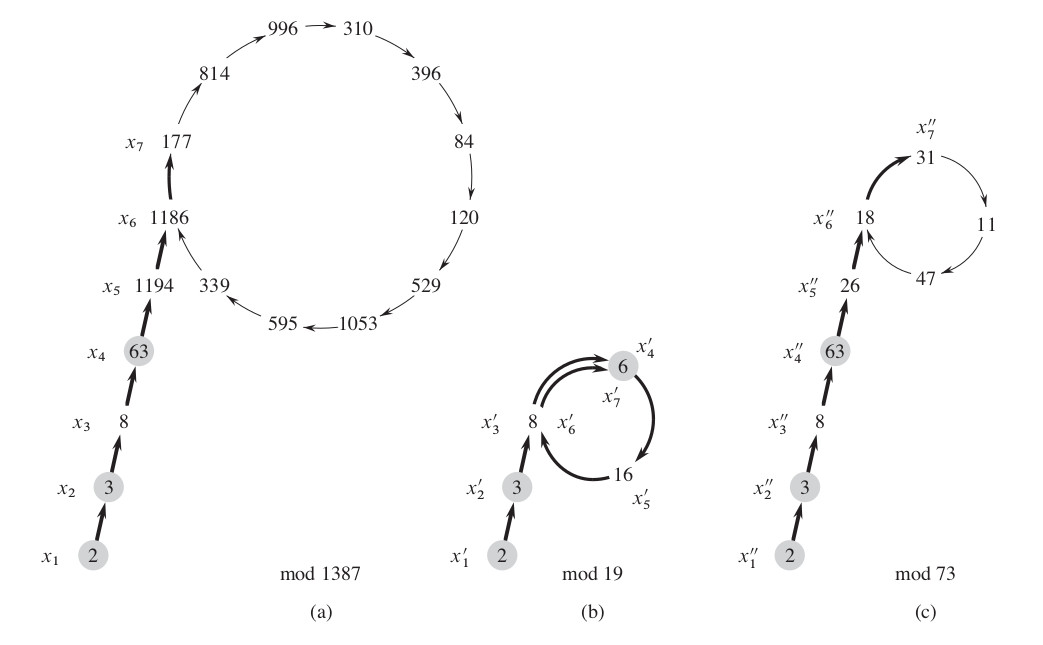
\includegraphics[width=0.7\textwidth]{pollard_rho.jpg}
\end{figure}
Potrebbe succedere che i valori $\lambda$ e $\sigma$ per più di una ``sequenza ombra'' siano tali che la ``scoperta'' di due iterate identiche avvenga nello stesso istante, se $n = p \cdot q$ con \textit{p} e \textit{q} primi fa si che le corrispondenti iterate $x_j$ e $x_{2^i}$ siano congruenti modulo \textit{p} e modulo \textit{q}. Questo implica che $x_j$ e $x_{2^i}$ sono anche congrui modulo \textit{n} e dunque $gcd(x_j, x_{2^i}) = n$ questo ovviamente \textbf{non aiuta}. Nel caso di scomposizione $n = p^k$ può risutare semplicemnte che $z_{2^i} = z_j \Rightarrow x_{2^i} = x_j$ e anche in questo caso non si scopre nulla. L'efficienza è data da $p < \sqrt{n} \Rightarrow \mathcal{O}(\sqrt[4]{n})$ operazioni su numeri di $\mathcal{O}(\log{n})$ bit. 